\section{Optimising Abstract Graph Size}
\par \indent
As we have observed in lemmas \ref{aha-lemma:maxedgesincluster} and \ref{aha-lemma:maxtransitions}, the initial abstraction algorithm attempts to represent every optimal path between clusters and inside clusters.
However, most maps have far simpler topographies than the worst-case; in our  experimental scenarios we often observed the same path returned for different pairs of $(c, s)$ parameters when discovering intra-edges.
This presents us with an opportunity to compact the graph by removing unnecessary duplication from the abstract edge set. 
\par \indent
Consider the initial abstraction in Figure \ref{aha-fig:strongdominance}(a) and contrast it with our desired result in Figure \ref{aha-fig:strongdominance}(b). 
$\lbrace E3, E5 \rbrace$ represent the same path between nodes $w$ and $y$ but are annotated with different clearance values. 
The same is true  for $\lbrace E4, E6 \rbrace$ which both cover nodes $u$ and $y$. 
In such cases we say that $E3$ and $E4$ are \emph{strongly dominant}, which we denote $E3 \succ E5$ and $E4 \succ E6$. 
This is an irreflexive and asymmetrical relationship between edges which we formalise as: 
\begin{theorem}
\label{aha-theorem:strongdominance}
Let $\lbrace e_{a}, e_{b} \rbrace \in E_{abs}$ be two distinct edges which connect the same pair of abstract nodes and are annotated with capabilities $c_{a} \subseteq c_{b}$ such that: 
% AB: I removed the 1 \geq condition below
%$$ 1 \geq cv(e_{a}, c_{a}) \geq cv(e_{b}, c_{b}) \wedge weight(e_{a}) = weight(e_{b})$$
$$ cv(e_{a}, c_{a}) \geq cv(e_{b}, c_{b}) \wedge weight(e_{a}) = weight(e_{b})$$
Then $e_{a} \succ e_{b}$ and we may remove $e_{b}$ from $E_{abs}$ without loss of generality or optimality.
\end{theorem}
\begin{proof}
% need extra stuff to explain why e_{b} can never be longer thab e_{a} if capability dominance holds?
Since $c_{a} \subseteq c_{b}$, it must be the case that any agent with the correct capability to traverse $e_{b}$ must be likewise able to traverse $e_{a}$.
Further, if $cv(e_{a}, c_{a}) \geq cv(e_{b}, c_{b})$ holds, it must also be the case that any agent large enough to traverse $e_{b}$ is also large enough to traverse $e_{a}$.
These conditions are sufficient to preserve generality.
Finally, since $e_{a}$ is equal in weight to $e_{b}$, we cannot lose optimality by removing $e_{b}$.
\end{proof}
We term the resultant graph in which all strongly dominant edges have been removed a \emph{high-quality} abstraction.  

\begin{figure}[htbp]
	\vspace{-4pt}
        \begin{center}
                        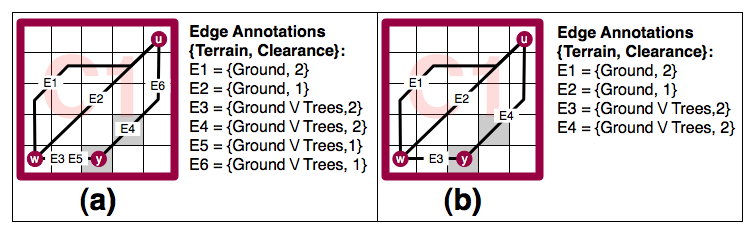
\includegraphics[scale=0.33, trim = 20mm 5mm 20mm 0mm]{diagrams/intraedges_initial.png}
        \end{center}
	\vspace{-7pt}
        \caption{(a) A cluster in an initial abstraction. (b) The same cluster once strong edge dominance is applied. \vspace{0.5em} }
        \label{aha-fig:strongdominance}
	\vspace{-7pt}
\end{figure}
A further observation made during our analysis of this problem was that in many cases there exist multiple alternative routes to reach a goal location.
The shortest paths tended to involve the traversal of optimal-length multi-terrain edges. However, it was often possible to reach the same destination using slightly longer single-terrain edges.
This suggests that the abstract graph can be further compacted without affecting the completeness of the representation.
\par \indent
In Figure \ref{aha-fig:abstractgraph}(a) and \ref{aha-fig:abstractgraph}(b) we show a typical high quality abstraction while in Figure \ref{aha-fig:abstractgraph}(c) and \ref{aha-fig:abstractgraph}(d) we highlight the desired result after further compacting the graph.
\begin{figure}[htbp]
	\vspace{-3pt}
        \begin{center}
                        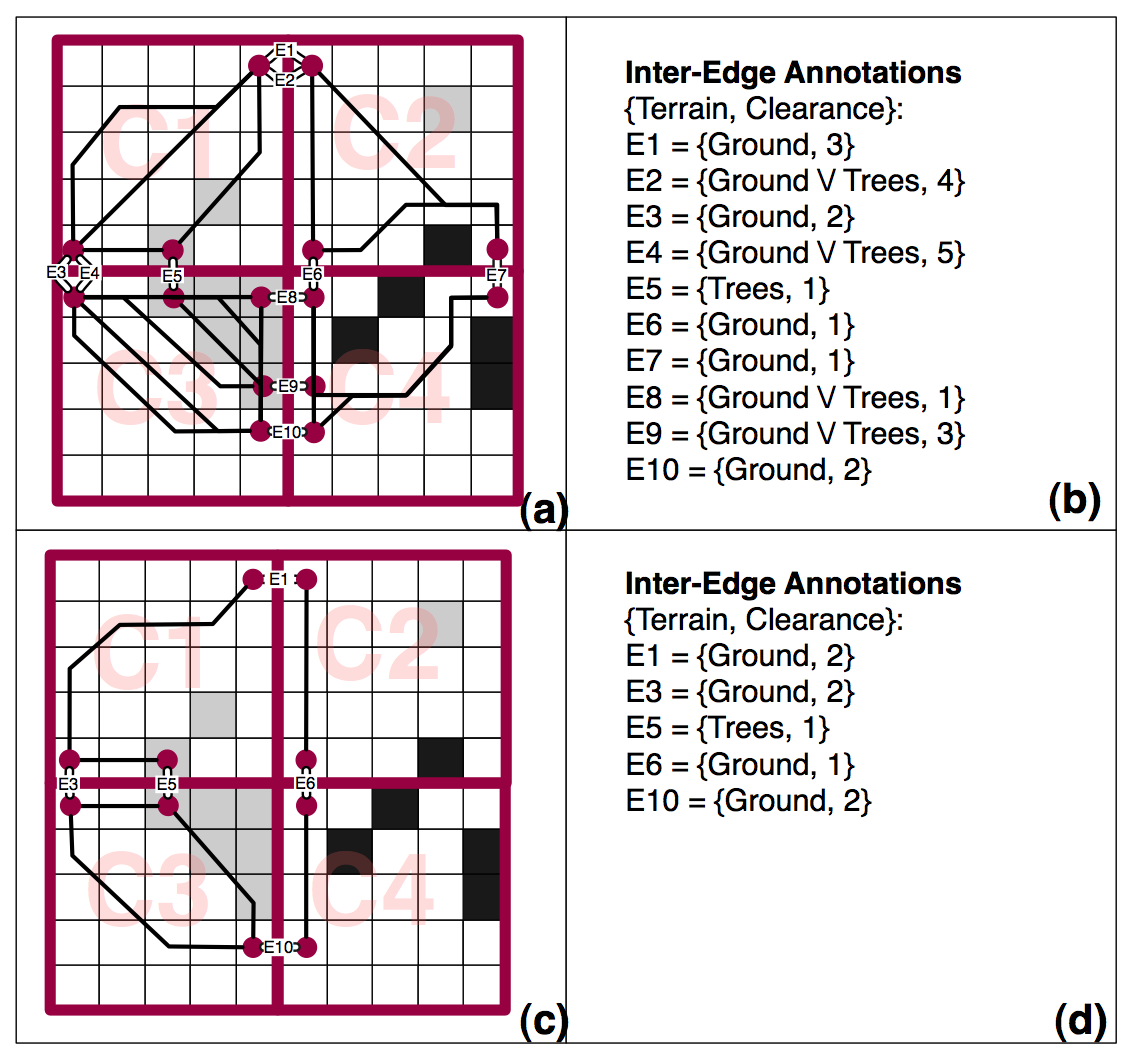
\includegraphics[scale=0.25, trim = 20mm 12mm 20mm 0mm]{diagrams/abstraction_result.png}
        \end{center}
	\vspace{-4pt}
        \caption{(a) A high quality abstraction of our toy map; note that some edges overlap and are not uniquely visible. (b) Inter-edges associated with the high quality graph. (c) The resultant graph after applying weak dominance. (d) Inter-edges associated with the low-quality graph.  \vspace{0.5em} }
        \label{aha-fig:abstractgraph}
	\vspace{-7pt}
\end{figure}
In this example we can see that, although edges $E1$ and $E2$ have different traversal requirements, any agent of size $s \in \lbrace 1, 2 \rbrace$ capable of traversing $E2$ can also traverse $E1$ without loss of generality. 
In such cases we say $E1$ is \emph{weakly dominant} and denote it as $E1 \succsim E2$. 
Notice also that $E3 \succsim E4$, $E6 \succsim E7$, $E10 \succsim E8$ and $E10 \succsim E9$.
\par \indent
%AB: I remove the next sentence as E6 and E7 seem to be in a symmetric relationship of weak domm.
%As with theorem \ref{aha-theorem:strongdominance}, this relationship is irreflexive and asymmetric.
Unlike the case of strong dominance, only representational completeness (and not optimality) is retained. 
We formalise it as:
\begin{theorem}
\label{aha-theorem:weakdominance}
Let $L_{a}$ and $L_{b}$ be two adjacent clusters, and $\lbrace w_{a}, x_{b} \rbrace, \lbrace y_{a}, z_{b} \rbrace \in V_{abs}$ two pairs of abstract nodes, each pair connecting $L_{a}$ and $L_{b}$.
Denote the inter-edges associated with these node pairs as $\lbrace e_{wx}, e_{yz} \rbrace \in E_{abs}$ and suppose they are annotated with clearance values $cv(e_{wx}, c_{wx}), cv(e_{yz}, c_{yz}) : c_{wx} \subseteq c_{yz} \in C$.
%Further, assume there exists an intra edge $e_{wy} \in E_{abs}$ connecting nodes $w_{a}, y_{a}$ and another intra-edge $e_{xz} \in E_{abs}$ connecting $x_{a}, y_{a}$.
 In this scenario, $e_{wx} \succsim e_{yz}$ iff the following conditions are met:
\begin{enumerate}
\item{The clearance dominance condition: $cv(e_{wx}, c_{wx}) \geq cv(e_{yz}, c_{yz})$}.
\item{The circuit condition: $\exists e_{wy}, e_{xz} \in E_{abs}$, annotated with the capabilities $c_{wy} \subseteq c_{yz}$ and $c_{xz} \subseteq c_{yz}$,
which connect $\lbrace w_{a}, y_{a} \rbrace$ and $\lbrace x_{b}, z_{b} \rbrace$ such that $cv(e_{wy}, c_{wy}) \geq cv(e_{yz}, c_{yz})$ and $cv(e_{xz}, c_{xz}) \geq cv(e_{yz}, c_{yz})$.}
\end{enumerate}
Then, any location which can be reached by traversing $e_{yz}$ can also be reached via $e_{wx}$.
\end{theorem}

\begin{proof}
If a circuit exists between the set of edges $\lbrace e_{wx}, e_{yz}, e_{wy}, e_{xz} \rbrace$ in which every edge is traversable by $c_{yz}$ with a clearance value at least equal to $cv(e_{yz}, c_{yz})$, then it follows that any nodes in $L_{a}$ or $L_{b}$ which are reachable from $y_{a}$ or $z_{b}$ must be reachable from $w_{a}$ or $x_{b}$.
Thus, any destination an agent can reach via $e_{yz}$ can also be reached via $e_{wx}$. 
\end{proof}

\begin{corollary}
If $e_{wx} \succsim e_{yz}$, then $y_{a}$ and $z_{b}$ and are also dominated and can be removed, unless required by another (non-dominated) inter-edge. 
\end{corollary}
\begin{proof}
If $y_{a}$ and $z_{b}$ are required by a non-dominated inter-edge, we cannot remove them without violating the clearance dominance condition which is required to retain representational completeness. 
If this is not the case however, we know by the circuit condition that any node reachable by an intra-edge via $y_{a}$ or $z_{b}$ is also reachable via the endpoints of $e_{wx}$. 
Thus, both nodes and any associated intra-edges dependent on them can be safely removed.
\end{proof}
In many situations, multi-terrain inter-edges tend to be associated with very large clearances; much larger than the size of our largest agent.
This unnecessarily limits the applicability of the clearance dominance condition from Theorem \ref{aha-theorem:weakdominance}. 
Leveraging the fact that $s_M = \max_{s \in S} s$ is known, we can maximise the number of edges which are weakly dominated by applying the following truncation condition to $E_{abs}$ before Theorem \ref{aha-theorem:weakdominance}:
$$
\forall e \in E_{abs} (cv(e, c_{e}) > s_M \Rightarrow cv(e, c_{e}) \leftarrow s_M) 
$$
%% DH: probably not required anymore? it's nice, but reads like filler.
%A reasonable analogy to highlight our intuition here is to compare the way off-road vehicles opportunistically use roads where possible even if an off-road route of trail exists which has a smaller distance cost.
%We prefer roads because they connect most points of interest, are smoother to drive on and have other benefits such as less wear and tear and better fuel consumption.
%\par \indent
Of course, opting for a low-quality abstraction in this way does affect the quality of computed solutions. 
In the worst case, a one-step transition of cost 1.0 in a high quality graph may be as long as $f(n) = 4n + f(n-2) : f(2) = 3, f(3) = 13$, where $n \geq 2$ is the length of a $n \times n$ cluster.
This is a pathological case however; as we will show the differences in real-world scenarios are much smaller and still near-optimal. 
The choice of which quality abstraction technique to employ will depend on the requirements of the specific application; it is a classic tradeoff between run-time performance vs space.
